
\documentclass[a4paper,12pt]{article}
\usepackage{mathtools}
\usepackage{tikz}
\usepackage{enumitem}
\usetikzlibrary{automata, positioning}

\title{Computer Science 350 \\
\large Assignment One}
\author{Steven Kerr 6022796}
\date{02/04/2019}

\begin{document}
\maketitle

\noindent \textbf{1.}
\texttt{is no output alphabet (d) \\
From class, a DFA is a five-tuple $M = (Q, \Sigma, \delta, s, F)$ \\
Where:}
\begin{enumerate}
	\item $Q$ is the finite set of machine states
	\item $\Sigma$ is the finite input alphabet
	\item $\delta$ is a transition function from $Q x \Sigma$ to $Q$
	\item $s \in Q$ is the start state
	\item $F \subseteq Q$ is the accepting state
\end{enumerate}
\texttt{There is no mention of an "Output alphabet" in the five-tuple DFA $\dots$ \newline}


\noindent \textbf{2.}
\texttt{The answer is 7. With the Kleene star on the alphabet $(0, 1)$ and with the string length being at most 2, we have: \\
$L=\{\epsilon, 0, 1, 00, 01, 10, 11\}$ \\
$|L|=7$\\ $\dots$ \newline}

\noindent \textbf{3.}
\texttt{(A) $input \in \Sigma^*$ Because of "input" being lowercase "i" \newline}

\noindent \textbf{4.}
\texttt{The set $(A^* \cap B) \cup (B^* \cap A)$ is equal to $\emptyset$ \\
for $A^* \cap B = \emptyset$\\
$=\{\epsilon, Hello, World, HelloWorld, HelloHello, \dots \} \cap \{Input, Output\} = \emptyset$ \\
for $B^* \cap A$ \\
$=\{\epsilon, Input, Output, InputOutput, InputInput, \dots \} \cap \{Hello, World\} = \emptyset$ \\
$\emptyset \cup \emptyset = \emptyset$ Therefore the set is the empty set \\ $\dots$ \\}

\noindent \textbf{5. \\}
\textbf{NFA M \\}
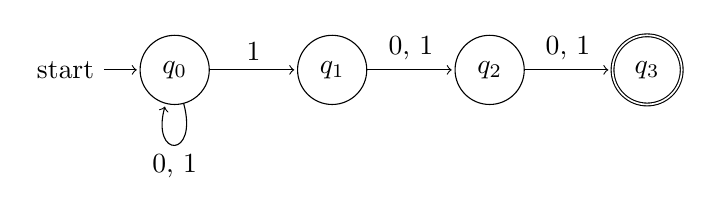
\begin{tikzpicture}[shorten >=1pt, node distance=2cm, on grid, auto]
	\node[state, initial] (q_0) {$q_0$};
	\node[state, right=of q_0] (q_1) {$q_1$};
	\node[state, right=of q_1] (q_2){$q_2$};
	\node[state, accepting, right=of q_2] (q_3) {$q_3$};
	
	\path[->]	
	(q_0) edge[loop below] node{0, 1} (q_0)
	(q_0) edge node{1} (q_1)
	(q_1) edge node{0, 1} (q_2)
	(q_2) edge node{0, 1} (q_3);
\end{tikzpicture}

\textbf{ \\ DFA N \\}
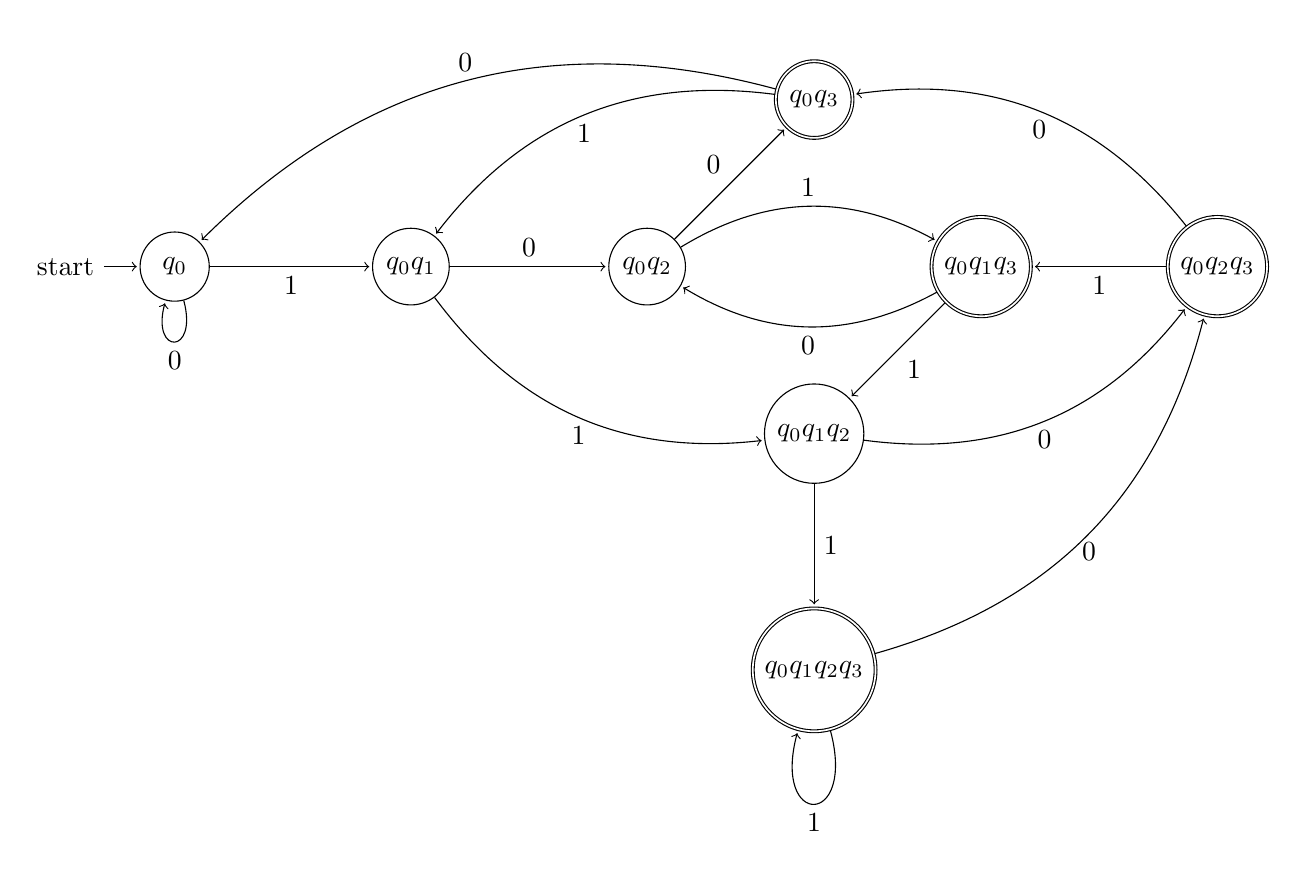
\begin{tikzpicture}[shorten >=1pt, node distance=3cm, on grid, auto]
	\node[state, initial] (A) {$q_0$};
	\node[state, right=of A] (B) {$q_0q_1$};
	\node[state, right=of B] (C){$q_0q_2$};
	\node[state, accepting, above right=of C] (D) {$q_0q_3$};
	\node[state, accepting, below right=of D] (F) {$q_0q_1q_3$};
	\node[state, accepting, right=of F] (G){$q_0q_2q_3$};
	\node[state, below right=of C] (E) {$q_0q_1q_2$};
	\node[state, accepting, below=of E] (H){$q_0q_1q_2q_3$};
	
	\path[->]	
	(A) edge[loop below] node{0} (A)
	(A) edge[below] node{1} (B)
	(B) edge node{0} (C)
	(B) edge[bend right, below] node{1} (E)
	(C) edge node{0} (D)
	(C) edge[bend left, above] node{1} (F)
	(D) edge[bend right, above] node{0} (A)
	(D) edge[bend right, below] node{1} (B)
	(E) edge[bend right, below] node{0} (G)
	(E) edge node{1} (H)
	(F) edge[bend left, below] node{0} (C)
	(F) edge node{1} (E)
	(G) edge[bend right, below] node{0} (D)
	(G) edge node{1} (F)
	(H) edge[bend right, below] node{0} (G)
	(H) edge [loop below] node{1} (H);
\end{tikzpicture}

\newpage

\noindent \textbf{6.}
\begin{enumerate}[label=\alph*)]
	\item $L=\{w \in \{ 0, 1 \} \: | \: w\: contains\: the\: substring\: 001\: \}$
	\item We notice that $L$ contains infinitely many strings, for example \\ $\{ (001)^n 				| n > 1 \} \in L$. we also notice that there are infinitely many strings not 				in $L$, for example $\{ (01)^n | n > 1 \} \notin L$. These are both infinitely 			large sets, however, one is in $L$ and the other is not.
	\item DFA M \\
	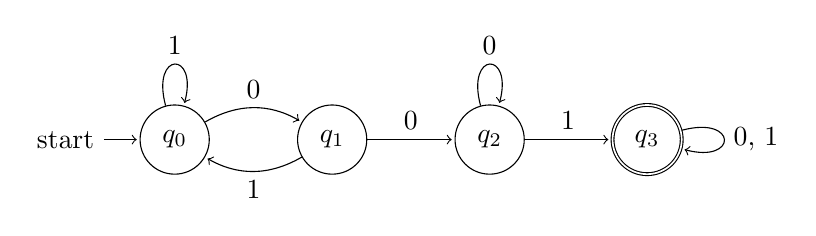
\begin{tikzpicture}[shorten >=1pt, node distance=2cm, on grid, auto]
	\node[state, initial] (q_0) {$q_0$};
	\node[state, right=of q_0] (q_1) {$q_1$};
	\node[state, right=of q_1] (q_2){$q_2$};
	\node[state, accepting, right=of q_2] (q_3) {$q_3$};
	
	\path[->]	
	(q_0) edge[loop above] node{1} (q_0)
	(q_0) edge[bend left, above] node{0} (q_1)
	(q_1) edge[bend left, below] node{1} (q_0)
	(q_1) edge node{0} (q_2)
	(q_2) edge[loop above] node{0} (q_2)
	(q_2) edge node{1} (q_3)
	(q_3) edge[loop right] node{0, 1} (q_3);
	\end{tikzpicture}
	\newline
	First we take $u \in L, u=\sigma_1 \dots \sigma_n , \sigma_{n+1} , \sigma_{n+2} , \dots \sigma_k$ where $\sigma_n , \sigma_{n+1} , \sigma_{n+2} = 001$. We take the sequence $r_0 \dots r_n , r_{n+1} , r_{n+2} , \dots , r_k$ where $r_i = q_0$ for $ 0 \geq i \geq n$, and $r_{n+2} = q_3$. Now we will show that this sequence of states is indeed an accepting trace of $u$ on DFA M. Observe that $r_0 = q_0 \in S$ and $r_{n+2} = q_3 \in F $. Further, note that $ r_n = q_1 \in \delta (r_{n-1} , \sigma_n ) = \delta ( q_0 , 0 )$,
	$ r_{n+1} = q_2 \in \delta (r_{n} , \sigma_{n+1} ) = \delta ( q_1 , 0 )$ ,
	$ r_{n+2} = q_3 \in \delta (r_{n+1} , \sigma_{n+2} ) = \delta ( q_2 , 1 )$.
	Notice this is the only trace to get to the accepting state, hence, $u$ is accepting by the DFA M. \\ \\
	Now we take $u \in L(M)$, $u=\sigma_1 \dots \sigma_n , \sigma_{n+1} , \sigma_{n+2} , \dots \sigma_k$ where $\sigma_n , \sigma_{n+1} , \sigma_{n+2} = 001$. Note that there is some trace $r_0 \dots r_n , r_{n+1} , r_{n+2} , \dots , r_k$ where $r_0 = q_0$, $r_n = q_1$ , $r_{n+1} = q_2$ and $r_{n+2} = q_3$. Note that: \\
	$r_{n+2} = q_3 \in \delta ( q_i , x )$ iff $q_i = q_2$ and $x = 1 = \sigma_{n+2}$ \\ and either\\
	$r_{n+1} = q_2 \in \delta ( q_i , x )$ iff $q_i = q_2$ and $x = 0 = \sigma_{n+1}$ \\
	$r_{n} = q_2 \in \delta ( q_i , x )$ iff $q_i = q_2$ and $x = 0 = \sigma_{n}$ \\
	Or \\
	$r_{n+1} = q_2 \in \delta ( q_i , x )$ iff $q_i = q_2$ and $x = 0 = \sigma_{n+1}$ \\
	$r_{n} = q_1 \in \delta ( q_i , x )$ iff $q_i = q_1$ and $x = 0 = \sigma_{n}$  \\
	
So, $run()=q_{0_{r_1}} \dots q_{0_{r_{n-1}}} q_1 q_2 q_3 \dots {q_3}^{k}$ so it must be the case that $u=(0,1)^j 001 (0,1)^k \in L$ \\
\item $L=(1+0)^* \cdot (001) \cdot (0+1)^*$

\newpage

\item So, in this case $P \: = \: 001$ and $A(P) = \{ u \: | \: u \: contains \: the \: pattern \: 001 \}$ and even further, $A(P)=\{u001v \: | \: u,v \in \{1, 0 \}^* \}$.

\item NFA N \\
	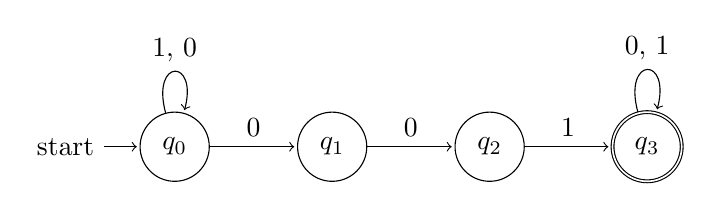
\begin{tikzpicture}[shorten >=1pt, node distance=2cm, on grid, auto]
	\node[state, initial] (q_0) {$q_0$};
	\node[state, right=of q_0] (q_1) {$q_1$};
	\node[state, right=of q_1] (q_2){$q_2$};
	\node[state, accepting, right=of q_2] (q_3) {$q_3$};
	
	\path[->]	
	(q_0) edge[loop above] node{1, 0} (q_0)
	(q_0) edge node {0} (q_1)
	(q_1) edge node{0} (q_2)
	(q_2) edge node{1} (q_3)
	(q_3) edge[loop above] node{0, 1} (q_3);
	\end{tikzpicture}
\newline
	
\item The number of states of the DFA and NFA are both the same however, the NFA has two less transition functions than the DFA. Mainly  $\delta ( q_2 , 0 ) = q_2$ and $\delta ( q_0 , 0 ) = q_1$. This means that the NFA is simpler than the DFA.

\end{enumerate}
\end{document}